\clearpage
\subsection{Reticolo: determinazione della lunghezza d'onda per diverse lampade}
Noto dal punto precedente il passo del reticolo di diffrazione, si utilizza lo stesso procedimento di misura per indagare lo spettro di emissione di gas incogniti, facendo sempre attenzione alla perpendicolarità del raggio incidente. Sono state utilizzate le lampade etichettate B,C,D. Di seguito i risultati.\\
\subsubsection{Lampada B}
Dati:
\begin{table}[H]
\begin{center}
\caption{Dati lampada D}
\begin{tabular}{|c|cc|}
\hline
Colore	&	$\sin \theta$	&	err $\sin \theta$	\\
	&	rad	&	rad	\\ \hline
Verde	&	0.329	&	0.003	\\
Arancione	&	0.347	&	0.003	\\
Viola1	&	0.255	&	0.003	\\
Viola2	&	0.262	&	0.003	\\ \hline
\end{tabular}
\end{center}
\label{label}
\end{table}

Risultlati:
\begin{table}[H]
\begin{center}
\caption{Spettro Lampada B}
\begin{tabular}{|c|c|c|}
\hline
Colore & Lungh.Onda [nm] & Errore [nm] \\ 
\hline
MassimoViola & 420 & 8 \\
\hline
Viola1 & 410 & 8 \\ 
Viola2 & 420 & 8 \\ 
Azzurro1 & 450 & 7 \\ 
Azzurro2 & 470 & 7 \\ 
Verde1 & 540 & 7 \\ 
Verde2 & 550 & 7 \\ 
Arancione & 600 & 7 \\ 
\hline
\end{tabular}
\end{center}
\label{label}
\end{table}

%
\subsubsection{Lampada C}
Dati:
\begin{table}[H]
\begin{center}
\caption{Dati lampada C}
\begin{tabular}{|c|cc|}
\hline
Colore	&	$\sin \theta$	&	err $\sin \theta$	\\
	&	rad	&	rad	\\ \hline
Giallo	&	0.351	&	0.004	\\ \hline
\end{tabular}
\end{center}
\label{label}
\end{table}

Risultati:
\begin{table}[H]
    \begin{center}
    \caption{Spettro lampada C}
    \begin{tabular}{|c|c|c|}
        \hline
        Colore & Lungh.Onda [nm] & Errore [nm]\\ 
        \hline
        Giallo & 590 & 7 \\ 
        \hline
    \end{tabular}
    \end{center}
    \label{table:O3_P2-2_sodio}
\end{table}


%
\subsubsection{Lampada D}
Dati:
\begin{table}[H]
\begin{center}
\caption{Dati lampada D}
\begin{tabular}{|c|cc|}
\hline
Colore	&	$\sin \theta$	&	err $\sin \theta$	\\
	&	rad	&	rad	\\ \hline
Massimo Viola	&	0.250	&	0.005	\\
Viola1	&	0.244	&	0.005	\\
Viola2	&	0.252	&	0.005	\\
Azzurro1	&	0.266	&	0.004	\\
Azzurro2	&	0.278	&	0.004	\\
Verde1	&	0.325	&	0.004	\\
Verde2	&	0.329	&	0.004	\\
Arancione	&	0.357	&	0.004	\\ \hline
\end{tabular}
\end{center}
\label{label}
\end{table}

Risultati:
\begin{table}[H]
    \begin{center}
    \caption{Spettro Lampada D}
    \begin{tabular}{|c|c|c|}
        \hline
        Colore & Lungh.Onda [nm] & Errore [nm]\\ 
        \hline
        Verde & 550 & 5 \\ 
        Arancione & 580 & 5 \\ 
        Viola1 & 430 & 5 \\ 
        Viola2 & 440 & 5 \\ 
        \hline
    \end{tabular}
    \end{center}
    \label{label}
\end{table}

%
%
\subsubsection{Confronto con spettro del visibile}
\label{sec:reticolo_confronto} 
%
% Spettro lampade B, C e D
%
    \begin{figure}[H]
    \centering
    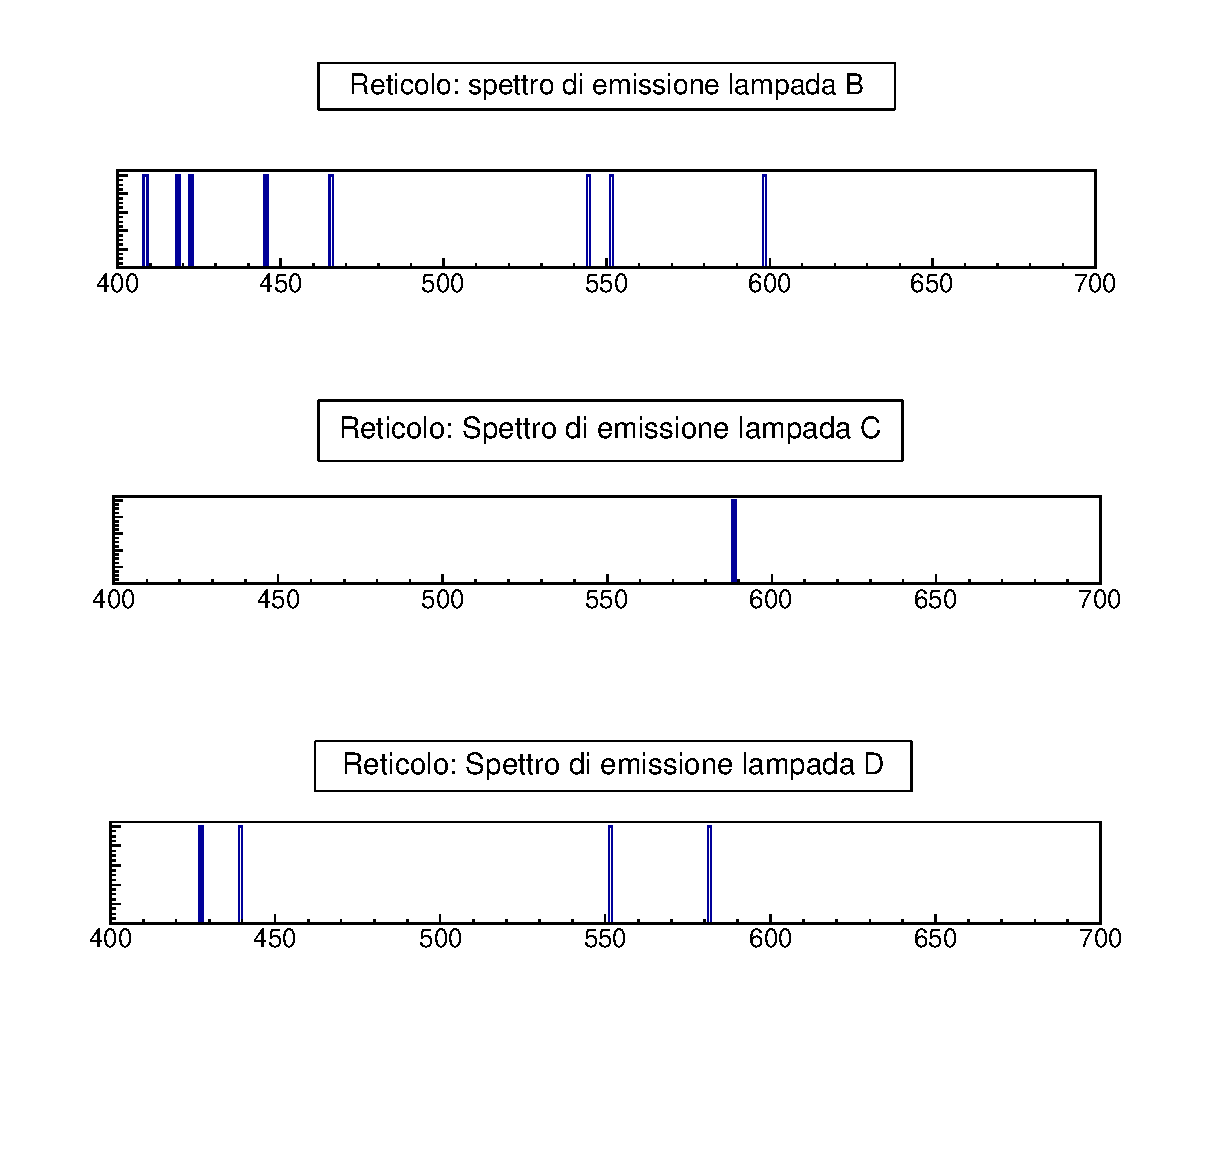
\includegraphics[scale=0.75]{Grafici/O3_P1_2_spectrum.eps}
%
    \includegraphics[scale=1.1]{Grafici/VISspectrum.jpg}
    %\caption{}
    \label{fig:C3_P2_RL}
    \end{figure} 
%